\documentclass{article}
\usepackage{amsmath}
\usepackage{graphicx}
\usepackage[margin=1in]{geometry}

\title{ Aerial Alumni \\ 2015  VWCC AUTONOMOUS ROBOTICS COMPETITION }
\author{ Jason Doyle \\ B.S. Electrical Engineering \\ VPI \& SU \and Phillip Benzinger \\ B.S. Computer Science \\ Liberty University }

\date{ \today }

\begin{document}

\maketitle

\begin{abstract}
Abstract goes here.
\end{abstract}
\clearpage

\tableofcontents
\listoffigures
\clearpage

% Remove this section from final report. Entered as a reminder of what is expected.
\section{ Technical Report: (Total = 60 pts) }
Each team must email ONE pdf document of its Technical Report (with all sections contained again in
one document) to George Studtmann (gstudtmann@virginiawestern.edu) by Friday, November 27 th ,
2013 by midnight. The Technical Report should include the components listed below. Each of the three
topics is worth 20 points.
\subsection{ Executive Summary: }
This summary should be no more than two pages using a 12-point font, single spaced, with 1-inch
margins. The summary should succinctly describe the problem that was solved, why the robot is an optimal
solution to the problem, and results of pre-competition testing.
\subsection{ CAD Images, Circuit Schematics, and Programming Flowcharts (or code): }
CAD images should adequately describe the form and function of the robot. Circuit schematics should
convey how the circuitry was constructed and how it works. A descriptive flowchart of the programming
code (or the code itself, if it is properly commented) should be provided.
\subsection{ Bill of Materials: }
The bill of materials should include the following information for each component of the robot: part
name, size or part number, vendor name, quantity used, unit price, and total price. You should also sum all
the total prices to display the overall cost of the components of your robot. This cost must be less than \$150
for components/items used outside of the BOE-bot kit. For components that you did not have to purchase,
you must still list a vendor where the item could be purchased along with the unit and total price. These
prices must be included in the overall cost of the robot.

\clearpage

\section{Introduction}

	The problem is to develop an autonomous robot to complete a set of trials. The first trial is.... The second .... third .... forth.... an autonomous air vehicle (AAV) was chosen to complete the trials. 
	
	The size of the robot can only be 8 in. x 12 in. x 10 in. high so a 250 size quad frame 
	was chosen. 250 represents 250 mm diagonal distance between the center of two propellers.
	The frame was also chosen because it has a frame built under it, to allow all of the
	electronics to be mounted.

\section{Conclusion}


\section{Future Work}

\section{Bill of Materials}

	\begin{tabular}{ l l l c r r }
		\textbf{Item} & \textbf{Item Num.} & \textbf{Store} & \textbf{Qty} & \textbf{Unit Price} & \textbf{Subtotal} \\ \hline
		Frame & 366000015-0 & Hobby King & 1 & \$19.99 & \$19.99 \\
		Motor CCW & 9536000002-0 & Hobby King & 2 & \$12.13 & \$24.26 \\
		Motor CW & 9536000001-0 & Hobby King & 2 & \$12.13 & \$24.26 \\
		Speed Controller & 9192000258-0 & Hobby King & 4 & \$12.99 & \$51.96 \\
		Power Distribution & 9171000530-0 & Hobby King & 1 & \$1.89 & \$1.89 \\
		Flight Controller & 9171000593-0 & Hobby King & 1 & \$24.99 & \$24.99 \\
		Gemfan Multirotor 10 Pair 6x4.5 Black & 329000381-0 & Hobby King & 1 & \$10.20 & \$10.20 \\
		Parallax Propeller Hat & 32230 & Parallax.com & 1 & \$24.95 & \$24.95 \\
		Electronic Mounting Plate & Custom Part & VWCC & 1 & TBD	& TBD \\
		Standoffs & & & 8 & & \\
		Wire & & & & & \\
		Connectors & & & & & \\
		Black Zip Ties & 0076328 & Lowes & 8 & X & X \\
		Thread Locker & 24200 & Lowes & N/A & N/A & N/A \\
		\hline
		\multicolumn{6}{ r }{\textbf{\$172.30}} \\ 
%	\end{tabular}
%
%	\subsection{Spare Parts}	
%	\begin{tabular}{ l l l c r r }
		\multicolumn{6}{ l }{\textbf{Spare parts}} \\
		\hline
		\textbf{Item} & \textbf{Item Num.} & \textbf{Store} & \textbf{Qty} & \textbf{Price} & \textbf{Subtotal} \\ \hline
		Speed Controller & 9192000258-0 & Hobby King & 2 & \$12.99 & \$25.98 \\
		Electronic Mounting Plate & Custom Part & VWCC & 1 & TBD	& TBD \\
		\hline
		\multicolumn{6}{ r }{\textbf{\$25.98}} \\ 
				
		\multicolumn{6}{ l }{\textbf{Shipping Costs}} \\ \hline
		\textbf{Shipper} & \textbf{From} &  &  &  & \textbf{Cost} \\ \hline
		EMS Express & \multicolumn{4}{ l }{Hobby King Int.} & \$38.47 \\
		Swiss Post Direct & \multicolumn{4}{ l }{Hobby King Int.} & \$2.46 \\
		USPS Priority Mail & \multicolumn{4}{ l }{Parallax Inc.} & \$7.15 \\
		\hline
		\multicolumn{6}{ r }{\textbf{\$48.08}} \\
		\cline{6-6}
		\multicolumn{5}{ r }{\textbf{Grand Total:}}  & \textbf{\$246.36}\\ 
	\end{tabular}
	
\section{Weight Budget}

	\begin{tabular}{ l c r r r r }
		\textbf{Item} & \textbf{Qty.} & \textbf{Unit Lift (g)} & \textbf{Unit Weight (g)}  & \textbf{Total Lift (g)} & \textbf{Total Weight (g)}\\ \hline
%		Speed Controller & 9192000258-0 & Hobby King & 2 & \$12.99 & \$25.98 \\
%		\hline
%		\multicolumn{6}{ r }{\textbf{\$000.00}} \\ 		
%		\multicolumn{6}{ l }{\textbf{Shipping Costs}} \\ \hline
%		\textbf{Shipper} & \textbf{From} &  &  &  & \textbf{Cost} \\ \hline
%		EMS Express & \multicolumn{4}{ l }{Hobby King Int.} & \$38.47 \\
%		Swiss Post Direct & \multicolumn{4}{ l }{Hobby King Int.} & \$2.46 \\
%		\hline
%		\multicolumn{6}{ r }{\textbf{\$000.00}} \\
%		\cline{4-6}
%		\multicolumn{5}{ r }{\textbf{Grand Total:}}  & \textbf{\$000.00}\\ 
	\end{tabular}
	
\clearpage

\section{CAD Drawings}

\begin{figure}[h!]
\caption{Electronics plate}
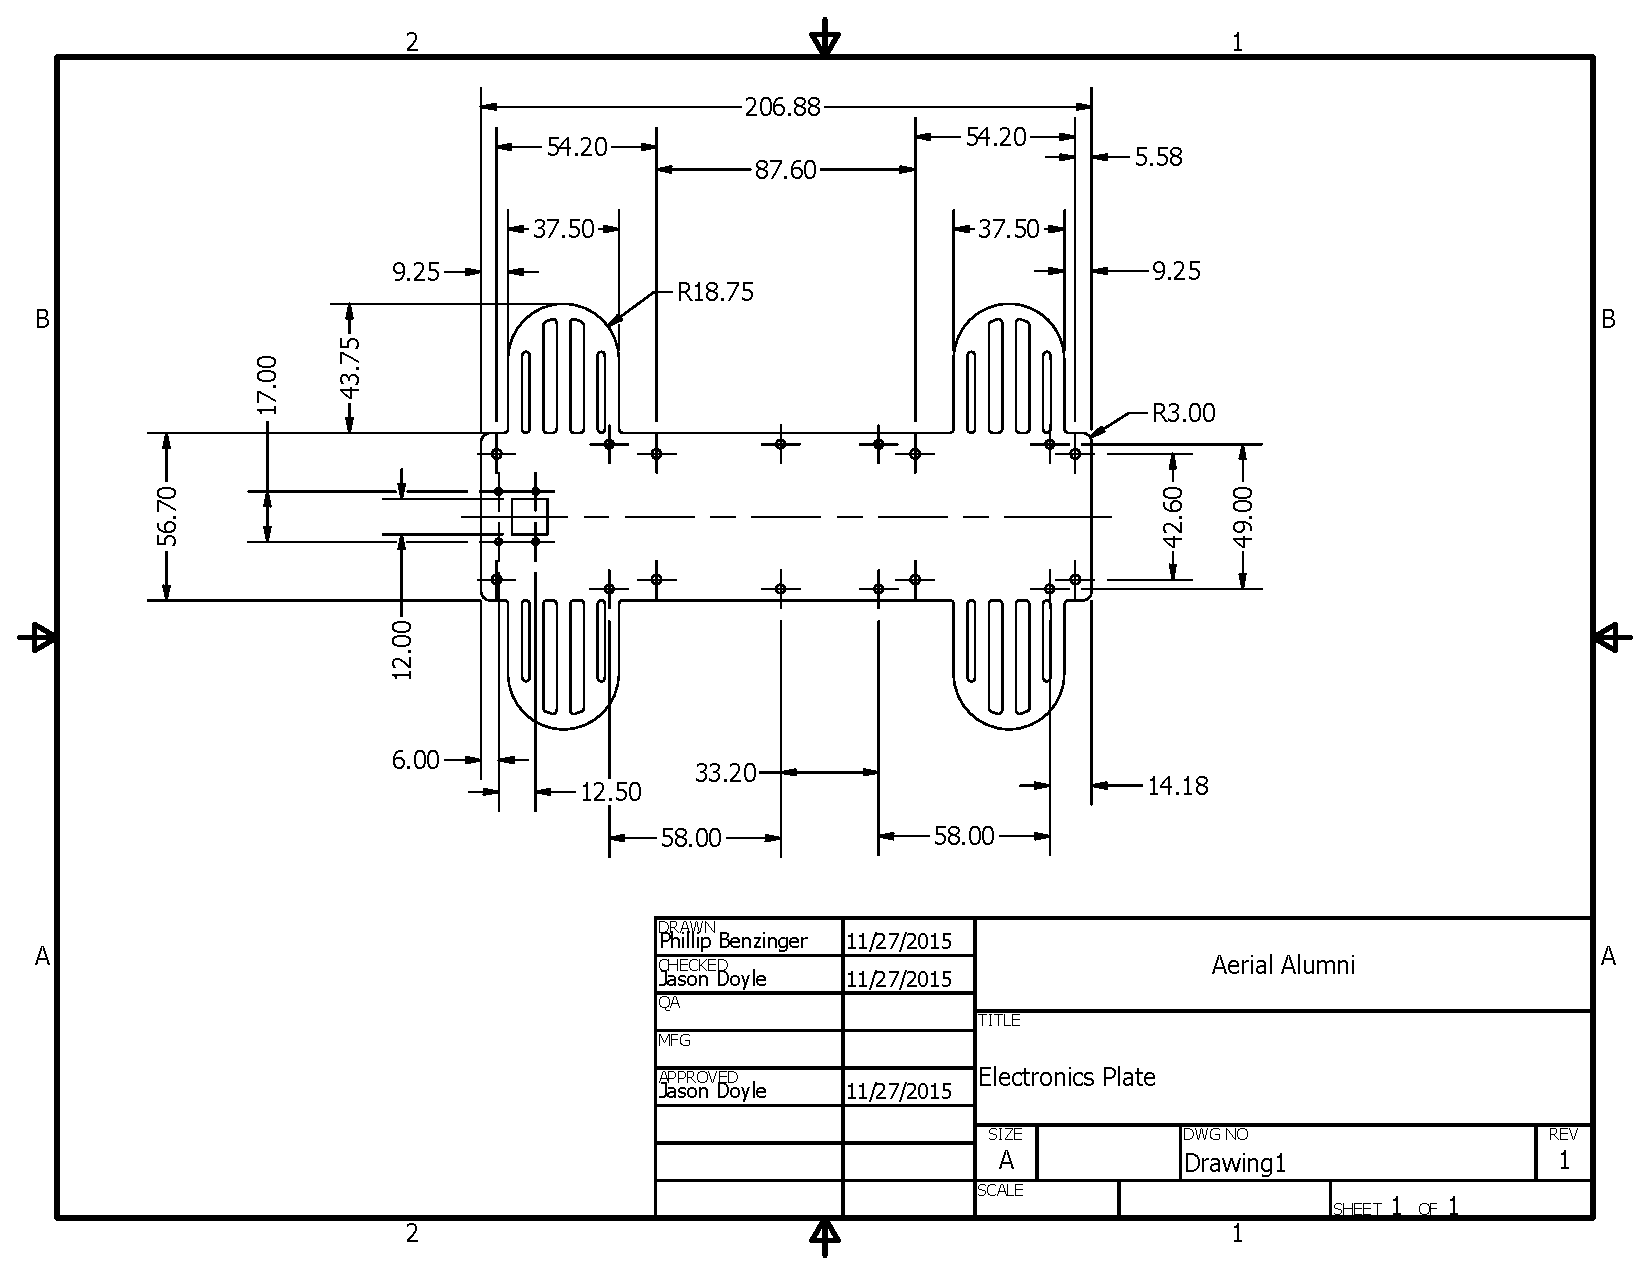
\includegraphics[scale=0.65, angle=90]{CAD.pdf}
\end{figure}

\begin{figure}[t]
\caption{Block Diagram}
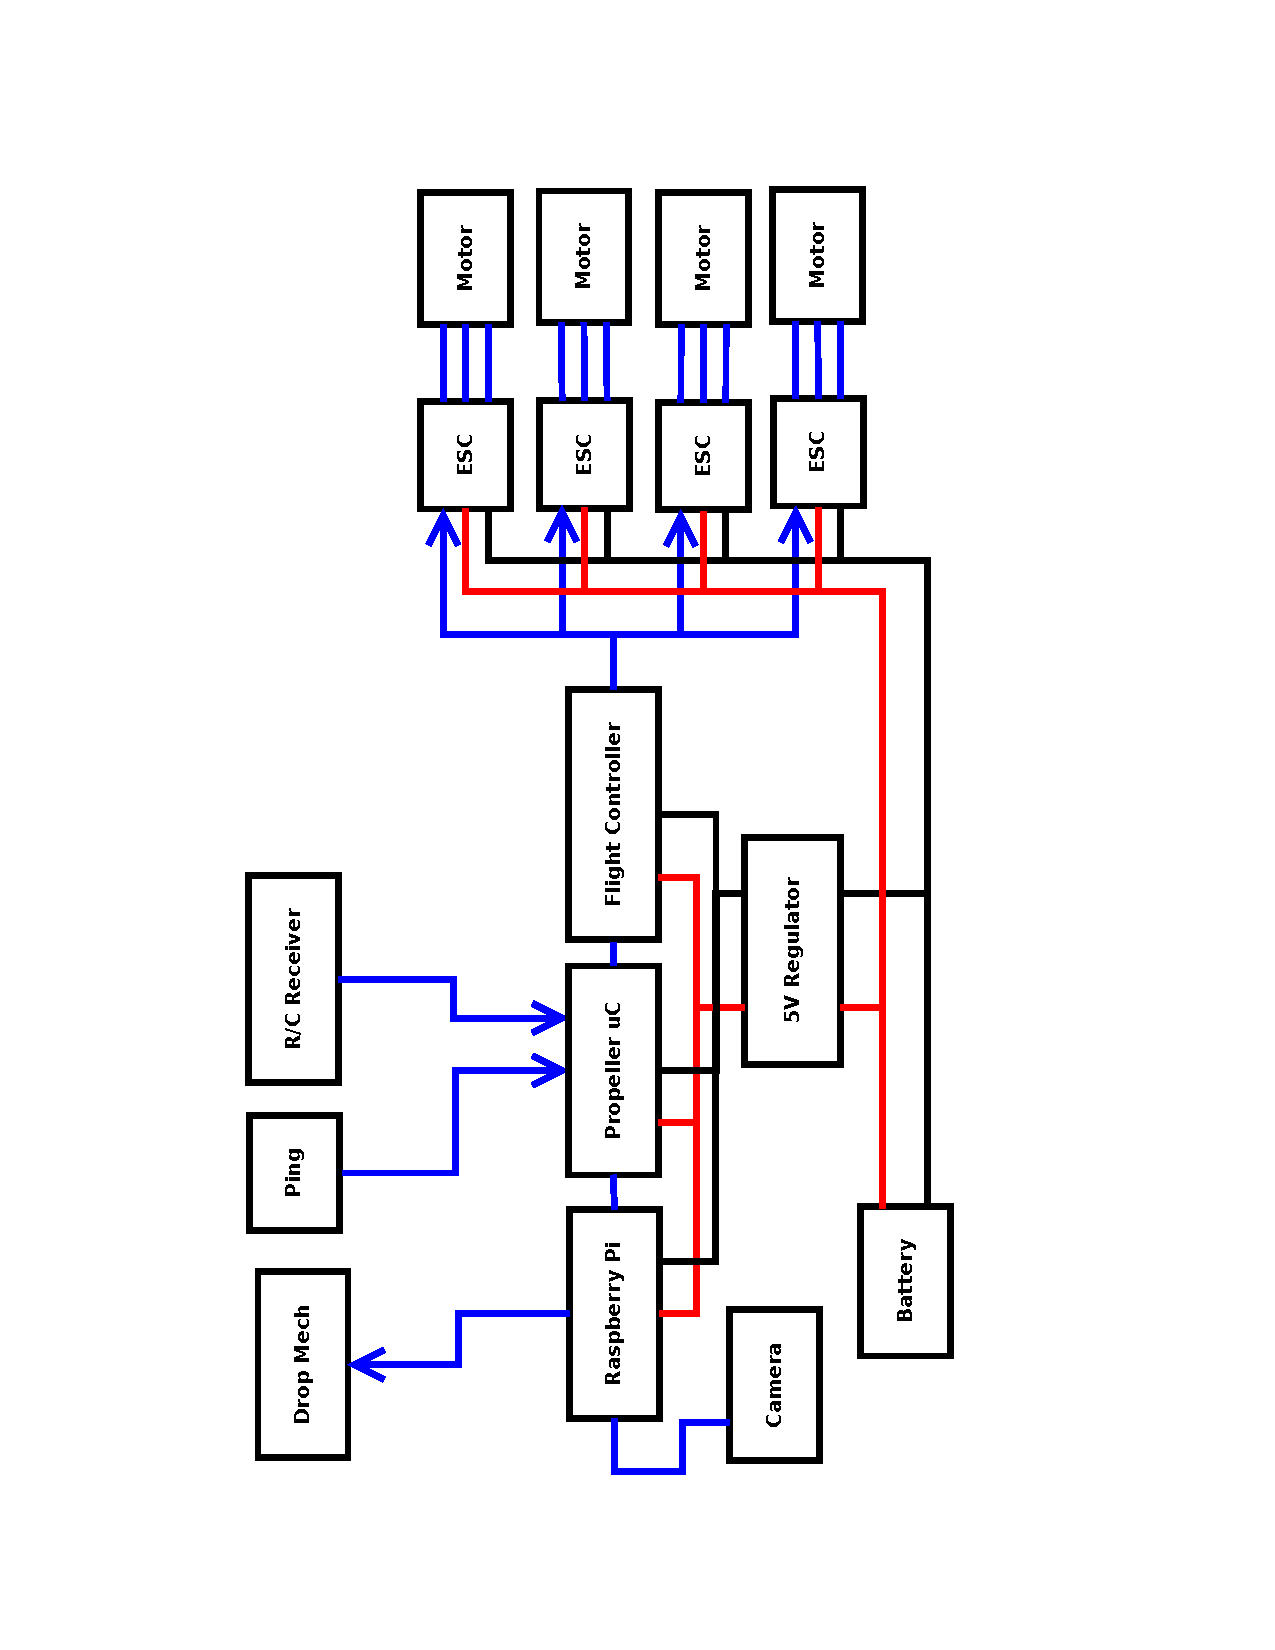
\includegraphics[width=\textwidth]{Block_Diagam_v2.pdf}
\end{figure}

\begin{figure}[t]
\caption{Propeller $\mu$C connections}
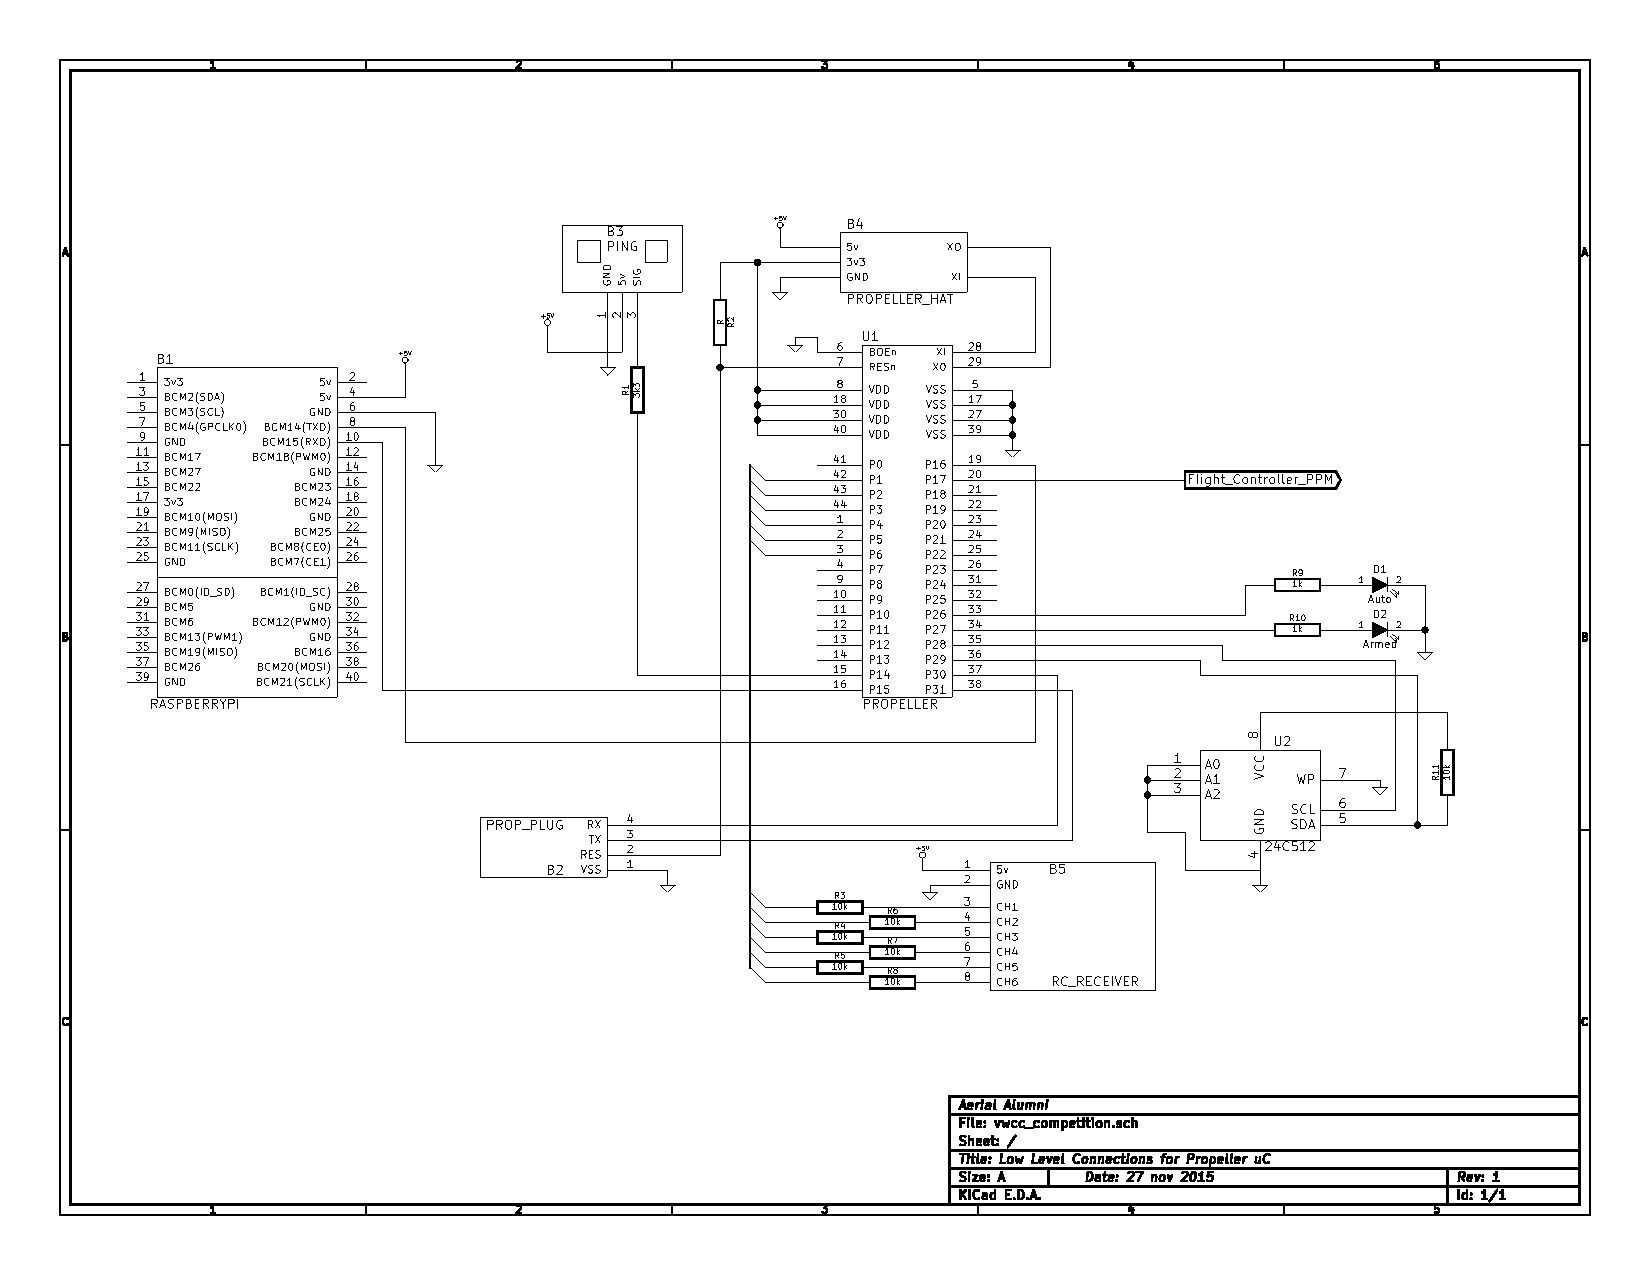
\includegraphics[height=\textwidth, angle=90]{vwcc_competition.pdf}
\end{figure}

\end{document}